\documentclass[12pt]{article}
\usepackage{amssymb}
\usepackage{graphicx}
\author{Blake Farman}
\title{Math-330: Homework 2}

\begin{document}
\maketitle
\newpage
\section*{5.2.1}
\(x^{'} = 4x-y, y^{'} = 2x + y\)

\subsection*{a)}
\begin{displaymath}
  J = \left[
  \begin{array}{cc}
    4 & -1\\
    2 & 1\\
    \end{array}
  \right]
\end{displaymath}

\begin{displaymath}
  \vec{x^{'}} = \left[
    \begin{array}{cc}
      4 & -1\\
      2 & 1\\
    \end{array}
    \right]
  \vec{x}
\end{displaymath}

\(tr(J) = 5\), \(det(J) = 6\)\\
\begin{eqnarray*}
  \lambda^2 - tr(J)\lambda - det(J) & = & \lambda^2 -5\lambda + 6\\
  &= & (\lambda - 3)(\lambda - 2)\\
\end{eqnarray*}

\subsection*{b)}

\(\lambda = 3\)
\begin{displaymath}
  \left[
    \begin{array}{cc}
      1 & -1\\
      2 & -2\\
    \end{array}
    \right]
  \left(
  \begin{array}{c}
    v_1\\
    v_2\\
  \end{array}
  \right)
  =
  \left(
  \begin{array}{c}
    0\\
    0\\
  \end{array}
  \right)
\end{displaymath}

\begin{displaymath}
  \Rightarrow\vec{v_1} = 
  \left(
  \begin{array}{c}
    1\\
    1\\
  \end{array}
    \right)
\end{displaymath}

\(\lambda = 2\)
\begin{displaymath}
  \left[
    \begin{array}{cc}
      2 & -1\\
      2 & -1\\
    \end{array}
    \right]
  \left(
  \begin{array}{c}
    v_1\\
    v_2\\
  \end{array}
  \right)
  =
  \left(
  \begin{array}{c}
    0\\
    0\\
  \end{array}
  \right)
\end{displaymath}

\begin{displaymath}
  \Rightarrow\vec{v_2} = 
  \left(
  \begin{array}{c}
    1\\
    2\\
  \end{array}
    \right)
\end{displaymath}

\begin{displaymath}
  \vec{x^{'}} = 
  c_1
  \left(
  \begin{array}{c}
    1\\
    1\\
  \end{array}
  \right)
  e^{3t}
  + c_2
  \left(
  \begin{array}{c}
    1\\
    2\\
  \end{array}
  \right)
  e^{2t}
\end{displaymath}

\subsection*{c)}
Unstable node.

\subsection*{d)}
\((x_0, y_0) = (3,4)\)

\begin{displaymath}
  \left(
  \begin{array}{c}
    8\\
    10\\
  \end{array}
  \right)
  = 
  c_1
  \left(
  \begin{array}{c}
    1\\
    1\\
  \end{array}
  \right)
  + c_2
  \left(
  \begin{array}{c}
    1\\
    2\\
  \end{array}
  \right)
\end{displaymath}

\begin{displaymath}
  \Rightarrow
  \vec{c} = 
  \left(
   \begin{array}{c}
     6\\
     2\\
   \end{array}
   \right)
\end{displaymath}

\begin{displaymath}
  \vec{x^{'}} = 
  6
  \left(
  \begin{array}{c}
    1\\
    1\\
  \end{array}
  \right)
  e^{3t}
  + 2
  \left(
  \begin{array}{c}
    1\\
    2\\
  \end{array}
  \right)
  e^{2t}
\end{displaymath}

\section*{5.2.3}

\(x^{'} = y\), \(y^{'} = -2x - 3y\)
\begin{displaymath}
  J = \left[
    \begin{array}{cc}
    0 & 1\\
    -2 & -3\\
    \end{array}
  \right]
\end{displaymath}
\(\lambda^2 +3\lambda + 2\)\\
\((\lambda+1)(\lambda+2))\)\\
\(\lambda=-1,-2\)\\
Stable node.\\
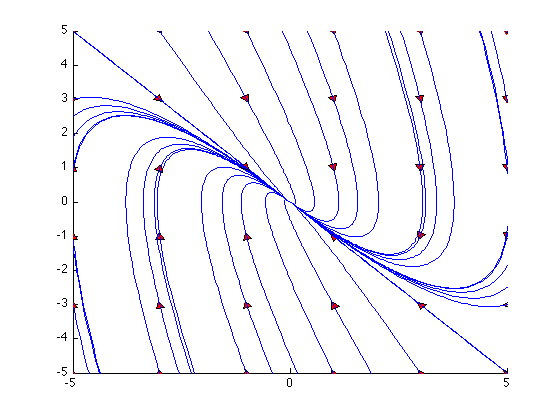
\includegraphics[scale=.5]{5-2-3.png}

\section*{5.2.5}

\(x^{'} = 3x-4y\), \(y^{'} = x-y\)
\begin{displaymath}
  J = \left[
  \begin{array}{cc}
    3 & -4\\
    1 & -1\\
    \end{array}
  \right]
\end{displaymath}
\(\lambda^2 + 2\lambda + +1\)\\
\((\lambda-1)(\lambda-1))\)\\
\(\lambda = 1,1\)\\
Unstable node.\\

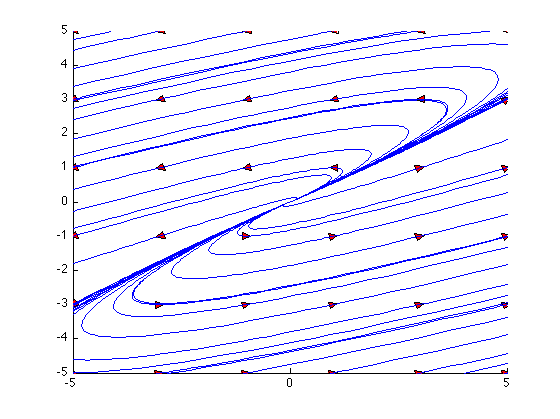
\includegraphics[scale=.5]{5-2-5.png}

\section*{6.3.6}

\(x^{'} = xy - 1\), \(y^{'} = x - y^3\)

\begin{displaymath}
  J = \left[
  \begin{array}{cc}
    y & x\\
    1 & -3y^2\\
    \end{array}
  \right]
\end{displaymath}

\(xy = 1 \Rightarrow x = \frac{1}{y}\)\\
\(\frac{1}{y} = y^3\)\\
\(\Rightarrow (x^{*}, y^{*}) = (1, 1)\), \((-1,-1)\)\\

\begin{displaymath}
  J_{(1,1)} = \left[
  \begin{array}{cc}
    1 & 1\\
    1 & -3\\
    \end{array}
  \right]
\end{displaymath}
\newpage
\(\lambda^2 + 2\lambda - 4\)\\
\begin{eqnarray*}
  \lambda & = & \frac{1}{2}(-2 \pm\sqrt{4 - 4(-4)}\\
  & = & \frac{1}{2}(-2 \pm2\sqrt{5})\\
  & = & (-1 \pm\sqrt{5})\\
\end{eqnarray*}
Saddle.\\
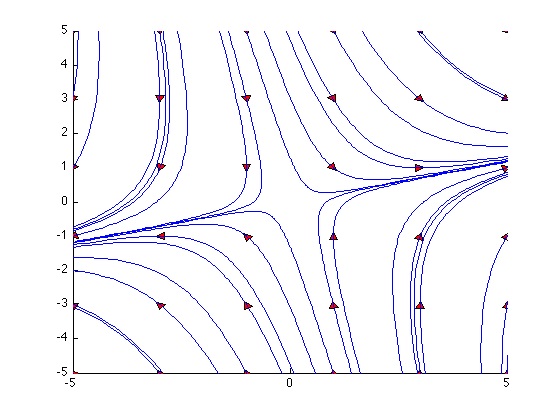
\includegraphics[scale=.5]{6-3-6a.png}
\newpage
\begin{displaymath}
  J_{(-1,-1)} = \left[
  \begin{array}{cc}
    -1 & -1\\
    1 & -3\\
    \end{array}
  \right]
\end{displaymath}
\(\lambda^2 + 4\lambda + 4\)\\
\((\lambda+2)(\lambda+2)\)\\
\(\lambda=-2,-2\)\\
Degenerate node.\\
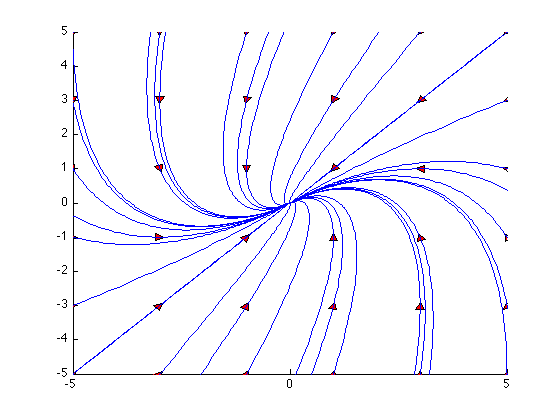
\includegraphics[scale=.5]{6-3-6b.png}
\newpage
\section*{6.4.3}
\(x^{'} = x(3-2x-2y)\),
\(y ^{'} = y(2-x-y)\)\\
\((x^{*},y^{*}) = (0,0), (\frac{3}{2},0), (0,2)\)

\begin{displaymath}
  J = \left[
  \begin{array}{cc}
    3-4x-2y & -2x\\
    -y & 2-x-2y\\
    \end{array}
  \right]
\end{displaymath}

\begin{displaymath}
  J_{(0,0)} = \left[
  \begin{array}{cc}
    3 & 0\\
    0 & 2\\
    \end{array}
  \right]
\end{displaymath}

\((\lambda-3)(\lambda-2)\)\\
\(\lambda=2,3\)
Unstable node.\\
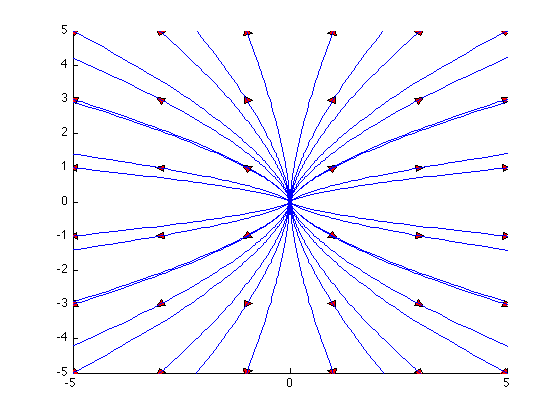
\includegraphics[scale=.5]{6-4-3a.png}
\newpage
\begin{displaymath}
  J_{(\frac{3}{2},0)} = \left[
  \begin{array}{cc}
    -3 & -3\\
    0 & \frac{1}{2}\\
    \end{array}
  \right]
\end{displaymath}

\(\lambda^2 + \frac{5}{2}\lambda -\frac{3}{2}\)\\
\((\lambda + 3)(\lambda - \frac{1}{2})\)\\
\(\lambda = -3,\frac{1}{2}\)\\
Saddle.\\

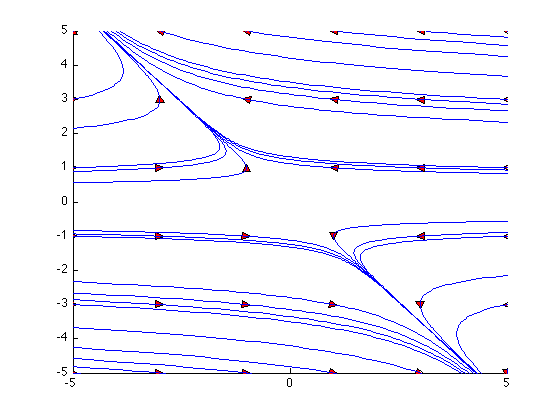
\includegraphics[scale=.5]{6-4-3b.png}
\newpage
\begin{displaymath}
  J_{(0,2)} = \left[
  \begin{array}{cc}
    -1 & 0\\
    -2 & -2\\
    \end{array}
  \right]
\end{displaymath}

\(\lambda^2 +3\lambda +2\)\\
\((\lambda + 2)(\lambda + 1)\)
\(\lambda = -2,-1\)\\
Stable node.\\

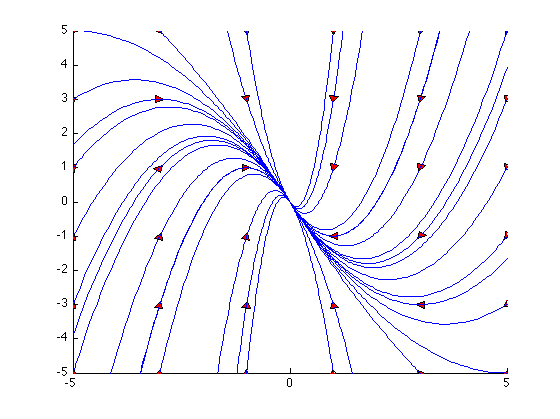
\includegraphics[scale=.5]{6-4-3c.png}
\end{document}
